% =============================================================================
%  Exposé – Bachelor Thesis
%  Real-time acoustic camera based on the miniDSP UMA-16 microphone array
%  Compile with: pdflatex -> biber -> pdflatex -> pdflatex  (Overleaf: default)
% =============================================================================
\documentclass[11pt,a4paper]{article}

% ---------------------------------------------------------------- packages ---
\usepackage[T1]{fontenc}
\usepackage[utf8]{inputenc}
\usepackage{lmodern}
\usepackage[english]{babel}
\usepackage[a4paper,left=2.5cm,right=2.5cm,top=2.5cm,bottom=2.5cm]{geometry}
\usepackage{amsmath,amssymb,bm}
\usepackage[per-mode=power]{siunitx}
\usepackage{booktabs,tabularx,array}
\usepackage{enumitem}
\usepackage{xcolor}
\usepackage{fancyhdr}
\usepackage{caption}
\usepackage{tikz}
\usetikzlibrary{positioning,arrows.meta,fit,calc,shapes.geometric}
\usepackage{pgfgantt}
\usepackage{csquotes}
\usepackage[backend=biber,style=ieee,doi=true,url=true]{biblatex}
\addbibresource{references.bib}
\usepackage[hidelinks]{hyperref}

\captionsetup{font=small,labelfont=bf}
\setlength{\parindent}{0pt}
\setlength{\parskip}{0.6em}
\setlist{itemsep=0.2em,topsep=0.3em}

% Placeholders that still have to be filled in are printed in red
\newcommand{\ph}[1]{\textcolor{red}{#1}}
\newcommand{\code}[1]{\texttt{#1}}

% ------------------------------------------------------------------ header ---
\pagestyle{fancy}
\fancyhf{}
\fancyhead[L]{Exposé -- Bachelor Thesis}
\fancyhead[R]{\ph{Your Name}}
\fancyfoot[C]{-- \thepage\ --}
\renewcommand{\headrulewidth}{0.4pt}
\setlength{\headheight}{14pt}
\fancypagestyle{plain}{\fancyhf{}\fancyhead[L]{Exposé -- Bachelor Thesis}%
  \fancyhead[R]{\ph{Your Name}}\fancyfoot[C]{-- \thepage\ --}}

% =============================================================================
\begin{document}

% -------------------------------------------------------------- title block ---
\begin{center}
  {\large\bfseries Technische Hochschule Würzburg-Schweinfurt (THWS)}\\[0.2em]
  Faculty of \ph{Electrical Engineering} -- Degree Programme International Mechatronics (IMC)\\[1.2em]
  {\Large\bfseries Exposé for the Bachelor Thesis}\\[1.0em]
  {\LARGE\bfseries Development and Evaluation of a Real-Time\\[0.3em]
   Acoustic Camera Based on a 16-Channel\\[0.3em]
   MEMS Microphone Array in Python}\\[1.2em]
  \begin{tabular}{@{}ll@{}}
    \toprule
    Author               & \ph{First name Last name} \\
    Matriculation number & \ph{0000000} \\
    Company / Institute  & \ph{Company or laboratory name, city} \\
    Academic supervisor  & \ph{Prof.\ Dr.-Ing.\ N.\,N.} \\
    Company supervisor   & \ph{N.\,N.\ (if applicable)} \\
    Planned period       & \ph{01.12.2026 -- 31.03.2027} \\
    Date                 & \today \\
    \bottomrule
  \end{tabular}
\end{center}

% =============================================================================
\section{Introduction}
% =============================================================================
An \emph{acoustic camera} combines a microphone array with an optical camera
and overlays a colour-coded map of sound pressure on the video image, so that
noise sources become literally visible. Acoustic cameras are used for noise
source identification on machines and vehicles, leak detection, quality
inspection in production and condition monitoring of mechatronic
systems~\cite{merino2019,christensen2004}. The underlying principle is
\emph{beamforming}: by compensating the different propagation times from a
point in space to each microphone, the array is electronically \enquote{focused}
on that point, and scanning a grid of points yields an acoustic
image~\cite{vanveen1988,benesty2008}.

Commercial acoustic cameras are expensive and closed systems. Low-cost MEMS
microphone arrays with a USB audio interface, such as the miniDSP UMA-16 with
16 synchronously sampled microphones~\cite{minidsp_uma16}, together with the
scientific Python ecosystem~\cite{harris2020} and open-source array-processing
libraries such as Acoular~\cite{sarradj2017}, now make it possible to build an
acoustic camera for teaching, prototyping and laboratory use at a fraction of
the cost. A first proof-of-concept that streams the UMA-16 into Python, computes
an acoustic map and blends it with a webcam image already exists. The
motivation of this thesis is to turn this prototype into a well-founded,
measurably validated real-time system and to understand its physical and
computational limits.

% =============================================================================
\section{Problem Definition}
% =============================================================================
The existing prototype consists of three independent scripts that implement
three different processing approaches:
(i) frequency-domain beamforming on a cross-spectral matrix with Acoular's
\code{BeamformerBase},
(ii) time-domain delay-and-sum beamforming with \code{BeamformerTime} on
octave-band pre-filtered signals, and
(iii) an own implementation of steered response power (SRP) based on
generalised cross-correlation, combined with an automatic gain control.
The approaches work qualitatively -- a hand clap is located on the video image
-- but the system has the following shortcomings:

\begin{itemize}
  \item \textbf{Real-time behaviour:} the frequency-domain variant re-creates
        the audio pipeline for every video frame, which leaves gaps in the
        audio stream and reaches only about \SI{5}{fps} at
        \SI{\approx 213}{\milli\second} latency. The time-domain variant reaches
        about \SI{20}{fps}, but audio acquisition and video capture run
        sequentially in the same loop and are not time-synchronised. The own
        SRP implementation evaluates every grid point and microphone pair in
        nested Python loops and is far from real-time.
  \item \textbf{Geometry and image registration:} the mapping between the
        acoustic grid and the camera image is set by hand (assumed field of
        view, image flips); the camera is not calibrated, and geometry
        parameters are defined inconsistently across the scripts.
  \item \textbf{No quantitative validation:} localisation accuracy, spatial
        resolution and the usable frequency range have never been measured.
        For a far-field rule of thumb, the \SI{126}{\milli\metre} aperture of
        the array gives a main-lobe width of roughly \SI{0.5}{\metre} at
        \SI{2}{\kilo\hertz} and \SI{0.3}{\metre} distance
        (Eq.~\eqref{eq:resolution}) -- much coarser than the
        \SI{1}{\centi\metre} grid spacing currently used suggests.
\end{itemize}

The thesis addresses the following research questions:

\begin{description}[leftmargin=3.2em,labelwidth=2.8em,font=\bfseries]
  \item[RQ1:] Which localisation method -- frequency-domain delay-and-sum,
        time-domain delay-and-sum with pre-filtering, or SRP-PHAT -- gives the
        best trade-off between localisation accuracy, spatial resolution and
        computational cost for the UMA-16 array?
  \item[RQ2:] How must the acquisition--processing--visualisation pipeline be
        structured (threading, buffering, vectorisation) so that the acoustic
        image is updated in real time without audio dropouts on a standard
        PC\ph{ (and on an embedded platform such as a Raspberry~Pi)}?
  \item[RQ3:] How closely do the measured spatial resolution and frequency
        limits of the array agree with the theoretical values, and how
        accurately can acoustic sources be registered to the camera image?
\end{description}

\textbf{In scope:}
\begin{itemize}
  \item Continuous, gap-free streaming of all 16 channels and a decoupled,
        time-stamped video capture.
  \item Implementation and comparison of the three localisation methods within
        one common, configurable software framework.
  \item Calibration of the camera and registration of the acoustic grid to the
        image plane.
  \item Experimental validation with loudspeakers at known positions,
        performance benchmarks and documentation.
\end{itemize}

\textbf{Out of scope:}
\begin{itemize}
  \item Development of hardware, firmware or new device drivers.
  \item Development of new beamforming theory; advanced deconvolution methods
        (e.g.\ DAMAS, CLEAN-SC) are considered only as an outlook.
  \item Absolute sound pressure calibration according to standards and moving
        sources.
\end{itemize}

% =============================================================================
\section{Objective Definition}
% =============================================================================
The thesis is considered successful when a single, documented Python
application exists that runs the acoustic camera in real time with a selectable
localisation method and fulfils the quantitative criteria in
Table~\ref{tab:objectives}. The acquisition requirements follow directly from
the number of channels $M$, the sampling frequency $f_s$, the sample word length
$b$ and the processing block length $N$:
\begin{equation}
  R = M \cdot f_s \cdot b = 16 \cdot \SI{48}{\kilo\hertz} \cdot \SI{32}{bit}
    \approx \SI{24.6}{\mega\bit\per\second},
  \qquad
  T_B = \frac{N}{f_s} = \frac{2048}{\SI{48}{\kilo\hertz}} \approx \SI{42.7}{\milli\second}.
  \label{eq:datarate}
\end{equation}
The UMA-16 delivers \SI{24}{bit} samples~\cite{minidsp_uma16}, which are
processed as 32-bit floating-point values. Every block of length $T_B$ must be
processed within $T_B$; for SRP on a $41\times41$ grid this means evaluating
$G \cdot M(M-1)/2 = 1681 \cdot 120 \approx 2\cdot10^{5}$ pair contributions per
block, which is only feasible with vectorised code.

\begin{table}[h]
  \centering
  \caption{Quantifiable success criteria (target values to be agreed with the supervisor).}
  \label{tab:objectives}
  \begin{tabularx}{\textwidth}{@{}lXr@{}}
    \toprule
    \textbf{No.} & \textbf{Criterion} & \textbf{Target value} \\
    \midrule
    O1 & Continuous streaming of all 16 channels at \SI{48}{\kilo\hertz} without dropped blocks & $\geq \SI{30}{\minute}$ \\
    O2 & Update rate of the acoustic overlay on a standard PC & $\geq \SI{15}{fps}$ \\
    O3 & End-to-end latency (sound event $\rightarrow$ displayed heatmap) & $\leq \SI{150}{\milli\second}$ \\
    O4 & Localisation error for a single source at \SI{1}{\metre} distance, \SIrange{1}{4}{\kilo\hertz} & $\leq \SI{5}{\centi\metre}$ \\
    O5 & Deviation of measured from theoretical $-\SI{3}{dB}$ main-lobe width & $\leq \SI{20}{\percent}$ \\
    O6 & Re-projection error of the camera calibration & $\leq \SI{1}{px}$ \\
    O7 & Speed-up of the SRP-PHAT implementation compared with the prototype & $\geq 20\times$ \\
    \bottomrule
  \end{tabularx}
\end{table}

% =============================================================================
\section{State of the Art}
% =============================================================================
\textbf{Signal processing.} Acoustic imaging with phased microphone arrays is
well established; a comprehensive review is given in~\cite{merino2019}, the
fundamentals in~\cite{benesty2008,brandstein2001,vanveen1988}. The basic method
is delay-and-sum beamforming. For a focus point $\mathbf{x}_g$ in the near
field and $M$ microphones at positions $\mathbf{r}_m$, the beamformer output is
\begin{equation}
  b(\mathbf{x}_g,t) = \frac{1}{M}\sum_{m=1}^{M} x_m\!\left(t + \tau_m(\mathbf{x}_g)\right),
  \qquad
  \tau_m(\mathbf{x}_g) = \frac{\lVert \mathbf{x}_g - \mathbf{r}_m \rVert}{c},
  \label{eq:das}
\end{equation}
where $c \approx \SI{343}{\metre\per\second}$ is the speed of sound. The same
operation can be carried out in the frequency domain on the cross-spectral
matrix, which allows narrow-band maps and averaging over many
blocks~\cite{christensen2004,sarradj2017}. In reverberant rooms,
SRP-PHAT~\cite{dibiase2001} is considered more robust: it sums the
phase-transform-weighted generalised cross-correlations~\cite{knapp1976}
$R_{mn}^{\mathrm{PHAT}}$ of all microphone pairs at the expected time
difference of arrival,
\begin{equation}
  P(\mathbf{x}_g) = \sum_{m=1}^{M-1}\sum_{n=m+1}^{M}
     R_{mn}^{\mathrm{PHAT}}\!\left(\tau_n(\mathbf{x}_g) - \tau_m(\mathbf{x}_g)\right).
  \label{eq:srp}
\end{equation}
The physical limits of an array follow from its aperture $D$ and microphone
spacing $d$. As a rule of thumb, the resolution at distance $z$ and the upper
frequency limit before spatial aliasing are
\begin{equation}
  \Delta x \approx 1.22\,\frac{z\,c}{f\,D},
  \qquad
  f_{\max} \approx \frac{c}{2d}.
  \label{eq:resolution}
\end{equation}
For the UMA-16 ($4\times4$ grid, $d = \SI{42}{\milli\metre}$,
$D = \SI{126}{\milli\metre}$~\cite{minidsp_uma16}) this gives
$f_{\max} \approx \SI{4.1}{\kilo\hertz}$, while low frequencies are limited by
the small aperture. Deconvolution methods such as DAMAS~\cite{brooks2006} and
CLEAN-SC~\cite{sijtsma2007} improve resolution, but at a high computational
cost. Overlaying the map on an image additionally requires a calibrated camera
model~\cite{zhang2000,bradski2000}.

\textbf{Software and systems.} Table~\ref{tab:software} compares existing
solutions. Commercial acoustic cameras offer real-time imaging but are costly
and closed. Acoular~\cite{sarradj2017} provides a comprehensive Python
framework for array processing, including a description of the UMA-16 geometry
and a live sound-card source, but is aimed at offline analysis.
pyroomacoustics~\cite{scheibler2018} focuses on simulation and DOA algorithms,
and ODAS~\cite{grondin2022} is an embedded C framework for localisation and
tracking without imaging. A transparent, real-time Python acoustic camera that
lets different methods be compared on the same hardware is therefore missing.
\ph{Add specific commercial products (e.g.\ manufacturer, price range) and check
Google Scholar, IEEE Xplore and the BeBeC proceedings for related low-cost
acoustic cameras.}

\begin{table}[h]
  \centering
  \caption{Qualitative comparison of selected existing solutions.}
  \label{tab:software}
  \small
  \begin{tabularx}{\textwidth}{@{}>{\raggedright}p{3.2cm}l>{\raggedright}X>{\raggedright\arraybackslash}X@{}}
    \toprule
    \textbf{Solution} & \textbf{Language} & \textbf{Main focus} & \textbf{Limitation for this thesis} \\
    \midrule
    Commercial acoustic cameras & -- & Industrial real-time acoustic imaging & Expensive, closed algorithms and hardware \\
    Acoular~\cite{sarradj2017} & Python & Beamforming, acoustic imaging & Offline-oriented, no camera overlay \\
    pyroomacoustics~\cite{scheibler2018} & Python & Room simulation, DOA algorithms & No real-time imaging or device layer \\
    ODAS~\cite{grondin2022} & C & Embedded localisation and tracking & No imaging, not a Python API \\
    Existing prototype & Python & Live overlay with UMA-16 & Not real-time capable, not validated \\
    \bottomrule
  \end{tabularx}
\end{table}

% =============================================================================
\section{Proposed Solution Approach}
% =============================================================================
The acoustic camera will be restructured into a modular, multi-threaded
pipeline (Figure~\ref{fig:architecture}). An acquisition thread continuously
reads blocks from the UMA-16 via PortAudio and the \code{sounddevice}
package~\cite{sounddevice}
into a ring buffer; a separate thread captures time-stamped video frames with
OpenCV~\cite{bradski2000}. A processing stage applies pre-processing (gain
normalisation, band-pass filtering) and one of three interchangeable
localisation back-ends. The resulting map is projected into the image using
the calibrated camera model and blended with the video frame.

\begin{figure}[h]
  \centering
  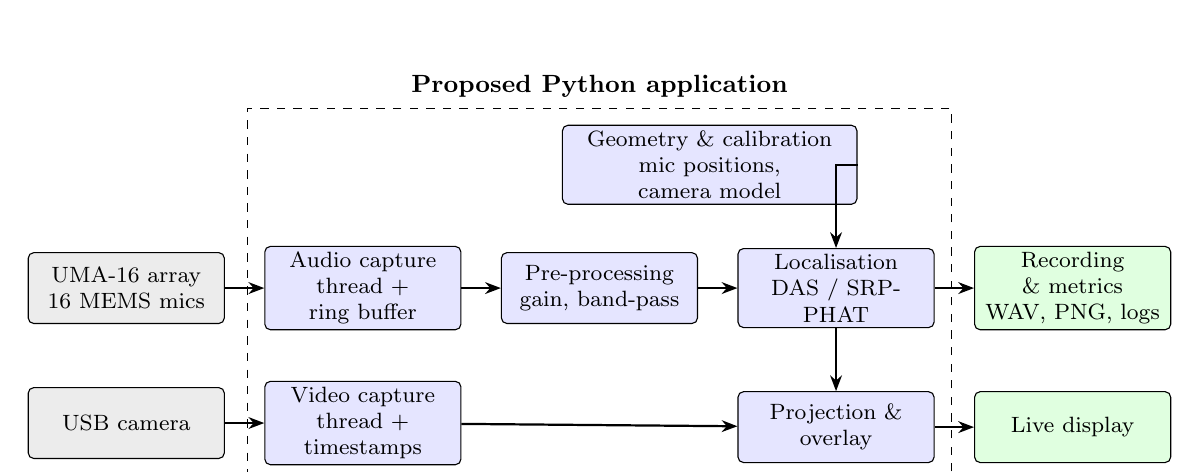
\begin{tikzpicture}[
      font=\footnotesize,
      box/.style={draw,rounded corners=2pt,align=center,minimum height=0.9cm,inner sep=2pt,text width=2.35cm},
      hw/.style={box,fill=gray!15},
      core/.style={box,fill=blue!10},
      outbox/.style={box,fill=green!12},
      arr/.style={-{Stealth[length=2mm]},thick}]
    % hardware
    \node[hw]  (mic) {UMA-16 array\\16 MEMS mics};
    \node[hw, below=0.8cm of mic] (cam) {USB camera};
    % software
    \node[core, right=0.5cm of mic] (acq) {Audio capture\\thread + ring buffer};
    \node[core, right=0.5cm of cam] (vid) {Video capture\\thread + timestamps};
    \node[core, right=0.5cm of acq] (pre) {Pre-processing\\gain, band-pass};
    \node[core, right=0.5cm of pre] (loc) {Localisation\\DAS / SRP-PHAT};
    \node[core, below=0.8cm of loc] (ovl) {Projection \&\\overlay};
    \node[core, above=0.6cm of pre, xshift=1.4cm, text width=3.6cm] (geo) {Geometry \& calibration\\mic positions, camera model};
    % outputs
    \node[outbox, right=0.5cm of ovl] (disp) {Live display};
    \node[outbox, right=0.5cm of loc] (exp) {Recording \& metrics\\WAV, PNG, logs};
    % frame
    \node[draw,dashed,inner sep=6pt,fit=(acq)(vid)(pre)(loc)(ovl)(geo),
          label={[font=\small\bfseries]above:Proposed Python application}] {};
    % arrows
    \draw[arr] (mic) -- (acq);
    \draw[arr] (cam) -- (vid);
    \draw[arr] (acq) -- (pre);
    \draw[arr] (pre) -- (loc);
    \draw[arr] (loc) -- (ovl);
    \draw[arr] (vid) -- (ovl);
    \draw[arr] (geo) -| (loc);
    \draw[arr] (ovl) -- (disp);
    \draw[arr] (loc) -- (exp);
  \end{tikzpicture}
  \caption{Planned architecture of the real-time acoustic camera.}
  \label{fig:architecture}
\end{figure}

The planned procedure follows an iterative engineering approach:
\begin{enumerate}
  \item \textbf{Analysis of the prototype:} profiling of the existing scripts
        (run time per stage, frame rate, dropped blocks) and derivation of
        functional and non-functional requirements (Table~\ref{tab:objectives}).
  \item \textbf{Hardware characterisation:} channel order and microphone
        geometry, inter-channel gain matching, supported sample rates and
        driver latency of the UMA-16.
  \item \textbf{Camera calibration and registration:} intrinsic calibration
        with a checkerboard~\cite{zhang2000}, measurement of the offset between
        camera and array centre, projection of the scan grid into the image
        instead of hard-coded flips and field-of-view values.
  \item \textbf{Architecture and implementation:} Python $\geq$ 3.10,
        \code{NumPy}, \code{SciPy}, \code{sounddevice}, \code{OpenCV} and
        \code{Acoular}; producer--consumer threads with a ring buffer;
        vectorised SRP-PHAT with pre-computed delay tables and fractional-delay
        interpolation; common interface for all three back-ends; Git for
        version control.
  \item \textbf{Verification and validation:} unit tests with simulated
        point sources (Eqs.~\eqref{eq:das}--\eqref{eq:srp}); measurements with a
        loudspeaker at known positions and frequencies
        (\SIrange{0.5}{4}{\kilo\hertz}) at several distances; determination of
        localisation error, main-lobe width (Eq.~\eqref{eq:resolution}), frame
        rate, latency (e.g.\ audio-visual clap test) and long-term stability.
  \item \textbf{Documentation:} README, installation guide and example
        configurations.
\end{enumerate}

% =============================================================================
\section{Draft Table of Contents}
% =============================================================================
\begin{enumerate}[label=\arabic*,leftmargin=1.2em,itemsep=0.5em]
  \item Introduction (motivation, problem statement, objectives, structure of the thesis)
  \item Fundamentals
    \begin{enumerate}[label=\theenumi.\arabic*,leftmargin=2em]
      \item Acoustics and MEMS microphone technology (sound field, sampling, synchronisation)
      \item Array signal processing (signal model, delay-and-sum, cross-spectral matrix, SRP-PHAT)
      \item Array performance (resolution, spatial aliasing, point spread function)
      \item Camera model and calibration
      \item Real-time audio processing on PCs (USB audio, PortAudio, buffering, threading)
    \end{enumerate}
  \item State of the Art and Related Work
  \item Analysis of the Existing Prototype and Requirements
  \item Concept and Architecture of the Acoustic Camera
  \item Implementation
  \item Verification and Validation
    \begin{enumerate}[label=\theenumi.\arabic*,leftmargin=2em]
      \item Test concept and simulation-based tests
      \item Measurement setup
      \item Localisation accuracy and spatial resolution
      \item Comparison of the localisation methods
      \item Real-time performance (frame rate, latency, CPU load)
    \end{enumerate}
  \item Discussion (fulfilment of objectives O1--O7, limitations)
  \item Summary and Outlook
\end{enumerate}
Appendix: measurement data, configuration reference, installation guide.

% =============================================================================
\section{Project Schedule}
% =============================================================================
Figure~\ref{fig:schedule} shows the planned schedule (\ph{adjust to your
official start and submission dates}). Milestones are marked with diamonds;
the last weeks are reserved as buffer before the submission deadline set by
the examination board.

\begin{figure}[h]
  \centering
  \begin{ganttchart}[
      hgrid, vgrid={*{17}{dotted}},
      x unit=0.42cm, y unit chart=0.5cm,
      title height=1,
      bar/.append style={fill=blue!25},
      bar label font=\footnotesize,
      milestone label font=\footnotesize\itshape,
      milestone/.append style={fill=red!60, shape=diamond, inner sep=2pt},
      title label font=\scriptsize,
    ]{1}{17}
    \gantttitle{Week}{17} \\
    \gantttitlelist{1,...,17}{1} \\
    \ganttbar{Literature review \& exposé}{1}{3} \\
    \ganttbar{Prototype analysis \& hardware}{2}{4} \\
    \ganttmilestone{M1: Requirements fixed}{4} \\
    \ganttbar{Camera calibration \& architecture}{5}{6} \\
    \ganttbar{Implementation \& optimisation}{6}{11} \\
    \ganttmilestone{M2: Real-time pipeline running}{9} \\
    \ganttbar{Measurements \& evaluation}{10}{14} \\
    \ganttmilestone{M3: Validation complete}{14} \\
    \ganttbar{Writing the thesis}{8}{16} \\
    \ganttbar{Buffer \& final corrections}{16}{17} \\
    \ganttmilestone{M4: Submission}{17}
  \end{ganttchart}
  \caption{Project schedule with milestones M1--M4.}
  \label{fig:schedule}
\end{figure}

\printbibliography

\end{document}
